\documentclass[10pt,a4paper,twocolumn]{ujarticle}
%upLaTeXを使用することを前提としています.
\setlength{\topmargin}{20mm}
\addtolength{\topmargin}{-1in}
\setlength{\oddsidemargin}{18mm}
\addtolength{\oddsidemargin}{-1in}
\setlength{\evensidemargin}{17mm}
\addtolength{\evensidemargin}{-1in}
\setlength{\textwidth}{174mm}
\setlength{\textheight}{254mm}
\setlength{\headsep}{0mm}
\setlength{\headheight}{0mm}
\setlength{\topskip}{0mm}

\makeatletter
\def\section{\@startsection {section}{1}{\z@}{2.0ex plus -1ex minus -.1ex}{0.5ex plus .1ex}{\normalsize\bf}}
\makeatother
\makeatletter
\def\subsection{\@startsection {subsection}{1}{\z@}{-3.5ex plus -1ex minus -.2ex}{2.3ex plus .2ex}{\normalsize\bf}}
\makeatother


\setlength{\columnsep}{2zw}
\renewcommand{\baselinestretch}{1}
\renewcommand{\thefootnote}{\fnsymbol{footnote}}
\pagestyle{empty}
%\usepackage{graphicx}
\usepackage[dvipdfmx]{graphicx}
\usepackage{bm}
\usepackage{multirow}
\usepackage{multirow}
\usepackage{amsmath}
\usepackage{amssymb}
\usepackage{amsfonts}
\usepackage{mathtools}
\begin{document}
\bibliographystyle{junsrt}

\twocolumn[%
\begin{center}
{\LARGE \textbf{自己注意によるコンテクスト抽出を用いた画像ノイズ除去手法}}\\
\flushright{\large 19C3020~有働~和矢}\\
\flushright{\large 指導教員~~宮田~高道~教授}\\
\vskip\Cvs
\end{center}
]

\section{背景}
画像ノイズ除去はノイズが発生した画像から, ノイズを含まない原画像を推定することを目的としている. 現在, 画像のノイズ除去においては深層畳み込みニューラルネットワーク(CNN)を用いる手法が一般的であるが, このような手法の問題点として, 畳み込み層の受容野が比較的狭く,長距離の画素間依存性を認識できないことが挙げられる. このため, 既存のCNNを用いた画像のノイズ除去手法では, 画像の持つコンテクスト(文脈情報)を判断することが困難であり, 除去すべきノイズと残すべき細部の特徴とを区別できないことが知られている.\\
 このような問題を解決するために, Transfomer\cite{SA}に代表される自己注意機構の利用が画像処理の分野で拡がっている. 自己注意機構は自然言語処理の分野で開発された長距離間の依存関係を認識できる手法であり, ノイズ除去に応用することで画像のコンテクストを把握しながらノイズ除去を行うことが可能となり, 高いノイズ除去性能が実現できることが明らかになっている. 一方で, コンテクスト抽出とノイズ除去の二つのタスクを異なる二種類のCNNで行うことで効率的にノイズ除去を行えるGTCNNとよばれる手法が提案されており\cite{GTCNN}, 画像ノイズ除去タスクにおいてコンテクストの把握とノイズ除去処理のすべてを自己注意機構のみで行うことは, CNNと同様に効率的でない可能性がある.\\
 前述のようにCNNにおけるノイズ除去は二種類のCNNを用いることで効率的に行うことができる. このうちコンテクスト抽出タスクを行うCNNを自己注意機構に置き換えることで, 既存手法と比較してより高いノイズ除去性能または効率的なノイズ除去性能を得ることを目的とする.
\section{関連研究}
\subsection{Gated context CNN}
Gated context CNN (以下GTCNN) は, 図\ref{fig:GTCNN_overall}に示すように入力層, 出力層, 中間層である$L$個のGCBR層(Gated CBR Layer)からなる. GCBR層はノイズ除去のみを行うCNN (CBR) とコンテクスト抽出のみを行うCNN (GTL) とに分離されている. GTLが抽出したコンテクストはゲート機構を介してCBRに渡されノイズ除去を制御する. このように機能分離を行うことで, 機能分離を行わない既存手法と比較して高いノイズ除去性能を獲得でき, またパラメータ数の削減に成功した. 
GTCNNのGTLはマルチスケール構造のU-Netをベースに設計されている. 

\begin{figure}[ht]
\centering
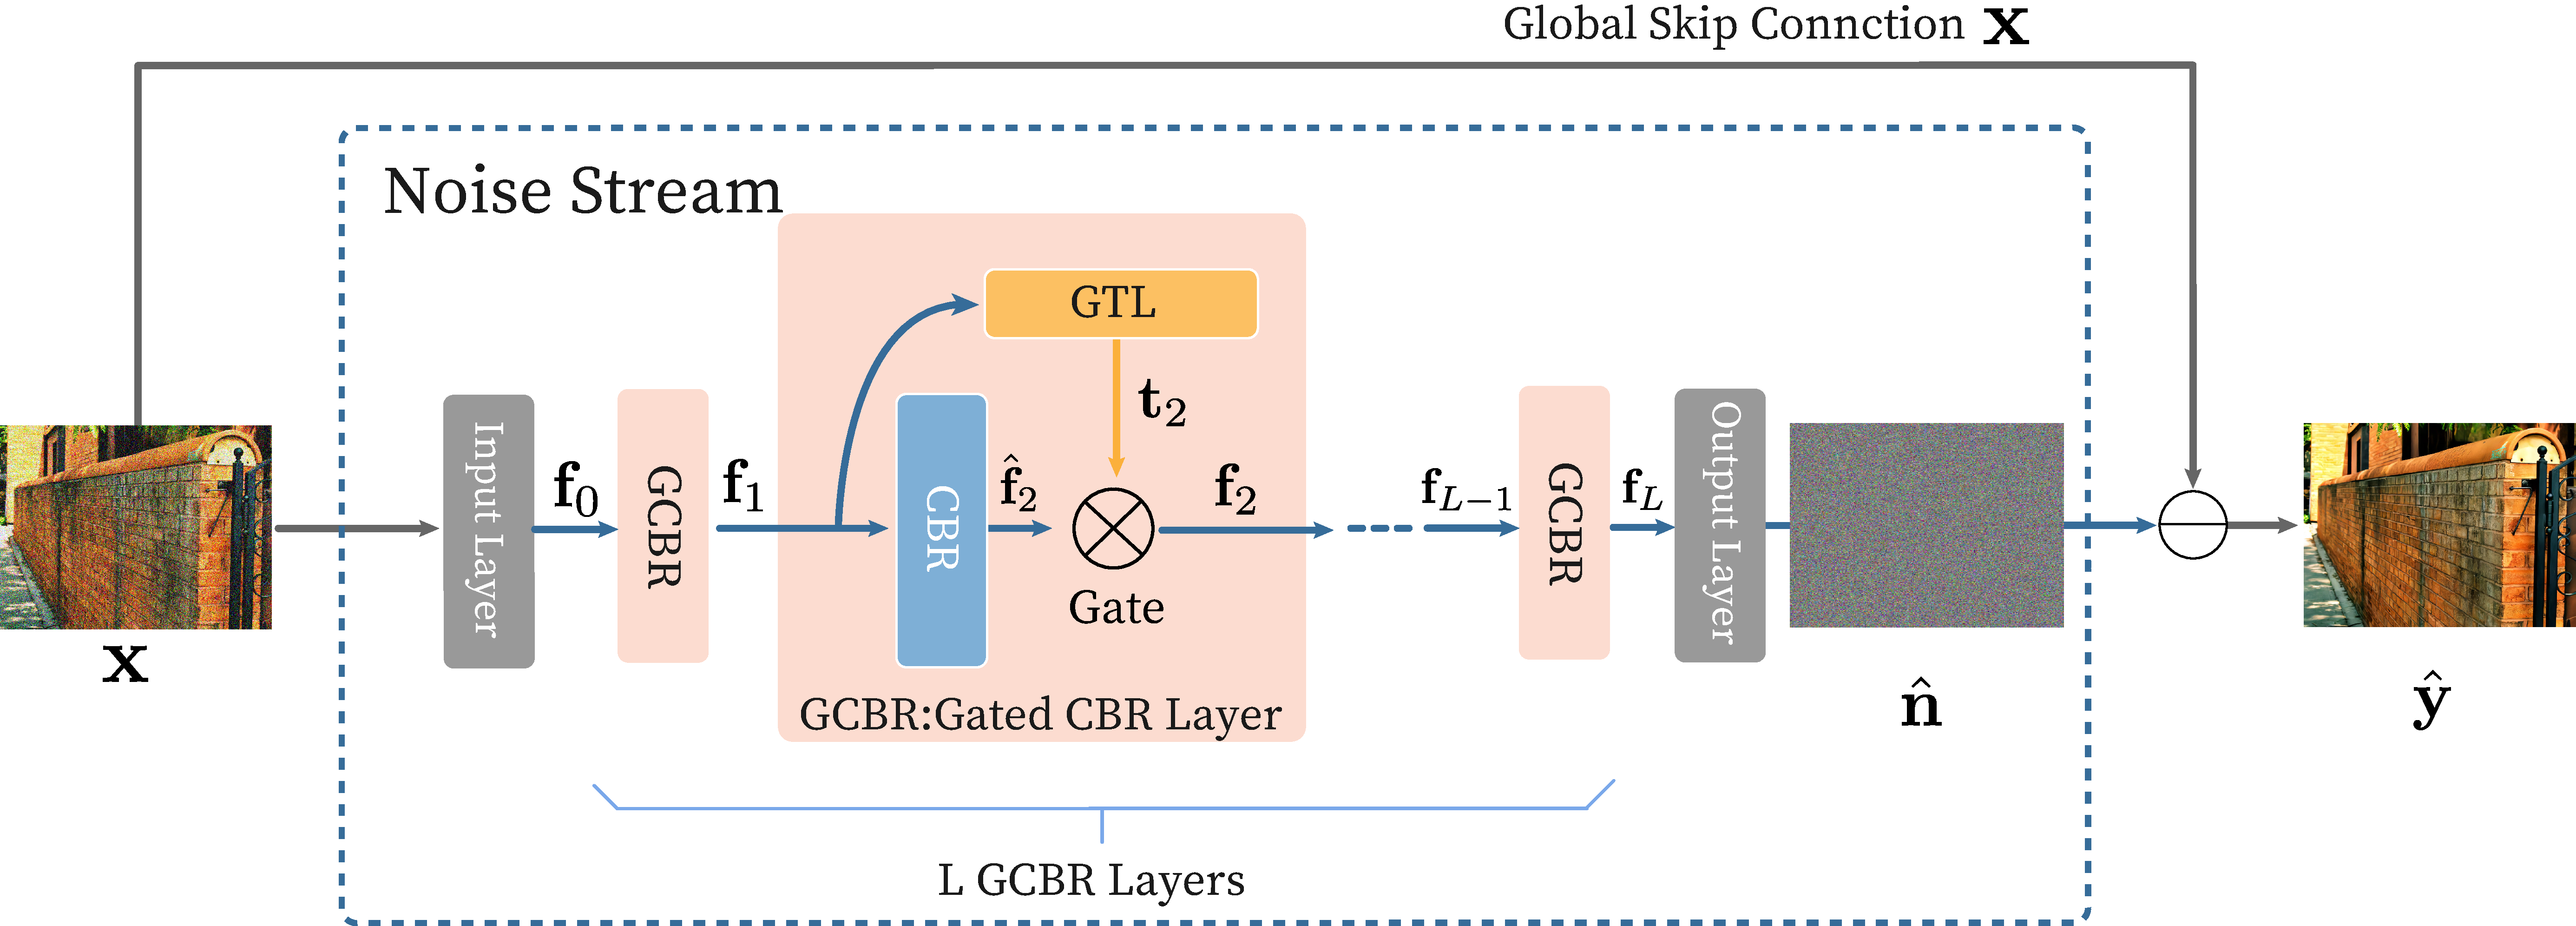
\includegraphics[scale=0.08]{figures/GTCNN_overall.pdf}
\caption{GTCNNのアーキテクチャ全体図. 文献\cite{GTCNN}より引用. (C) 2020 Springer \label{fig:GTCNN_overall}}
\end{figure}

\subsection{自己注意機構}
自己注意は式(\ref{eq:SA})のように表される\cite{SA}. $\mathbf{Q,K,V}$は入力にそれぞれ異なる埋め込み処理をしたものである.
\begin{align}
Attention(\mathbf Q,\;\mathbf K,\; \mathbf V)=softmax(\frac{\mathbf Q \mathbf K^T}{\sqrt{d_k}})\mathbf V \label{eq:SA}
\end{align}
 式(\ref{eq:SA})では$\mathbf{Q}$と$\mathbf{K}$から得られる全データ間の類似度をもとに, $\mathbf{V}$を処理することを表しており, このことから, 局所的な処理をするCNNとは異なり, 自己注意は大域的な処理を行っているといえる. Transformerを画像認識に応用したViT (Vison Transformer) ではこの特性のため, 広域なコンテクストの取得を可能とした. しかし自己注意機構には, 入力データ長の二乗に比例し計算量が増えてしまう課題が存在する. Restormer\cite{Restormer}はこの問題を解決するためにU-netに類似した構造を持つネットワーク構造と, 自己注意を画素位置ではなく特徴量のチャンネルに対して適用する転置自己注意を提案したが, ノイズ除去のすべてを自己注意で行うためにパラメータ数が増大することが課題であった.


\section{提案手法}
既存手法であるGTCNNにおいて, コンテクスト抽出を担うGTLはU-Netをベースに設計されている. 本論文ではGTLの各層にCNN以上にコンテクスト抽出にTransformerを組み込んだ手法, SAGTCNN (Self-Attention GTCNN) を提案する. Transformerを挿入する場所を変更したいくつかのバージョンを提案し, それらの性能を比較する. 実験を通して, Transformerのヘッドの数は1としている. 提案手法はGTLを変更した以外は従来のGTCNNのアーキテクチャを踏襲している.

\subsection{SAGTCNN-S4}
SAGTCNN-S4は図\ref{fig:GTL_S4}のような構造になっている. 青い枠の部分が従来手法に変更を加えたところである. 従来手法では全ての層がCNN Blockで形成されていたがSAGTCNN-S4では4段目をSA Blockに変更しているところに特徴がある. さらに, プーリングよるダウンサンプリングを畳み込みで行うようにし, バイリニアでのアップサンプリングを畳み込みで行うように変更した. SA Blockは畳み込みを2度行うD-conv層とAttention層の2層からなっている. Transformerは画像のスケールが大きくなるほど計算量が増大するため, スケールの小さい4段目でTransformerを用いることで計算量の増大を防いでいる. 

\begin{figure}[htbp]
\centering
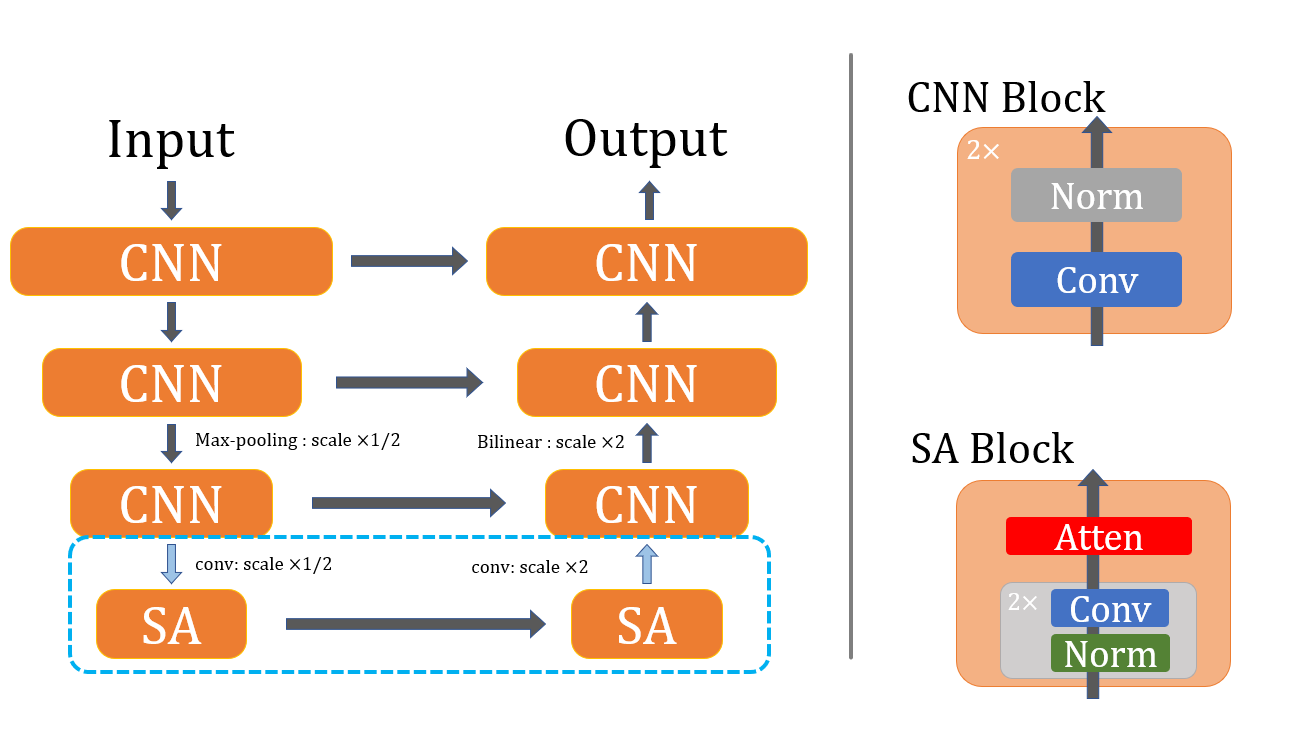
\includegraphics[scale=0.25]{figures/GTL_TS4.png}
\caption{SAGTCNN-S4のGTLのアーキテクチャ \label{fig:GTL_S4}}
\end{figure}

\section{実験}
提案手法の有効性を調べるため, 既存手法と提案手法のノイズ除去性能を比べた. その際, 生成ノイズを加算したグレースケール画像に対するノイズ除去性能を比較した. 本実験では, 既存手法GTCNNのCBR層の数を1つに固定した. 提案手法である自己注意機構を追加したGTCNN(Self-Attention GTCNN: 以後SAGTCNN)はGTLの4層目のCNNを自己注意に置き換えたSAGTCNN-S4, ミドル層に自己注意を追加したSAGTCNN-M, そのどちらの変更を加えたSAGTCNN-S4Mの3種類のパターンで比較を行った. GTCNNおよびSAGTCNNのGTLは共に4段で構成した.\\
 データセットにはDIV2Kを用いる. DIV2Kの全画像から$192 \times 192$画素のパッチをストライド192画素で切り出したものを学習画像とする. 学習のエポック数は600とする.\\
 既存手法と同様に, ノイズ除去評価手法において一般的に使われるガウシアンノイズを原画像に加算した画像(生成ノイズ画像)から原画像を推定する. ノイズ除去結果の評価はPSNRを用いる. 原画像にはSet12, BSD68, Urban100のデータセットを使用した. 従来手法であるGTCNNの評価値は, 論文に記載されている値を引用した.\\
 表\ref{tab:sigma30}に, ノイズの分散が$\sigma=30$のときのSAGTCNN-S4の結果を示す(これ以外の手法ならびに$\sigma$のときの結果は、卒業論文に記載する). この結果より, $\sigma=30$では提案するSAGTCNN-S4が従来手法であるGTCNNをわずかに上回る結果となった. 一方で, これ以外の手法や$\sigma$では, GTCNNの性能を上回ることが無いことも示された.


\begin{table}[htbp]
\centering
\caption{生成ノイズ$\sigma=30$におけるGTCNNとSAGTCNNの性能比較 \label{tab:sigma30}}
 \begin{tabular}{|l||c|c|c|}
 \hline
 手法 & Set12 & BSD68 & Urban100 \\ \hline \hline
 GTCNN         & 29.80 & $\bm{28.53}$ & 29.43 \\ \hline
 SAGTCNN-S4    & $\bm{29.81}$ & 28.52 & $\bm{29.46}$ \\ \hline
 \end{tabular}
\end{table}

\section{結論}
本論文では, GTCNNのコンテクスト抽出を行うGTLに自己注意機構を組み込んだ手法, SAGTCNNを提案した. 自己注意機構を挿入する場所を変更したSAGTCNN-S4, SAGTCNN-M, SAGTCNN-S4Mの3種類のパターンで実験を行った. 実験ではGTCNNに対しSAGTCNNは一部上回ったが, 明確な優位性を示すことができなかった. ノイズ除去性能の向上が見られなかった理由はいくつか考察できる. まず一般的に自己注意を用いる手法では大規模なデータセットを用いており, 今回の実験で使用した学習用のデータセットでは学習画像枚数が少ない可能性が考えられる. また, 己注意は広域のコンテクストを捉えることを得意とするが, 今回GTLの4段目という画像サイズの小さい領域でしか自己注意を用いておらず, 本来の性能が活かせなかったことが考えられる. 最後に画像に自己注意を用いる際にViTなどで行われている位置埋め込みを行っていないため, コンテクストの抽出が上手く行えなかった可能性が考えられる. \\
 今後の課題としては, 位置埋め込みの実装やリアルノイズでの性能比較, 自己注意をGTLの上層にて使用した際の有効性の検討などが挙げられる. 

{\small
\addcontentsline{toc}{chapter}{参考文献}
\bibliography{ref}
}
\end{document}
